% figures/src/setup_schematic.tex
% Standalone TikZ source for the conformal-antenna setup schematic.
% Rendered to figures/setup_schematic.pdf by paper-figures (pdflatex).
%
% This diagram is SCHEMATIC. The only annotated quantities are the ones recorded
% verbatim in benchmarks/patch_antenna_conformal/conformal_results.toml:
%   bend_radius_mm = 40, pml_thick_mm = 8, n_freeform_dofs = 73,
%   port_resistance_ohm = 50, band_omega = [0.3, 0.35, 0.4].
% All quantities are dimensionless / natural units. Do NOT relabel as GHz or mm.
% No geometry coordinates below are measured data; they are illustrative only.
\documentclass[tikz,border=4pt]{standalone}
\usepackage{amsmath}
\usetikzlibrary{arrows.meta,decorations.pathmorphing,calc}
\begin{document}
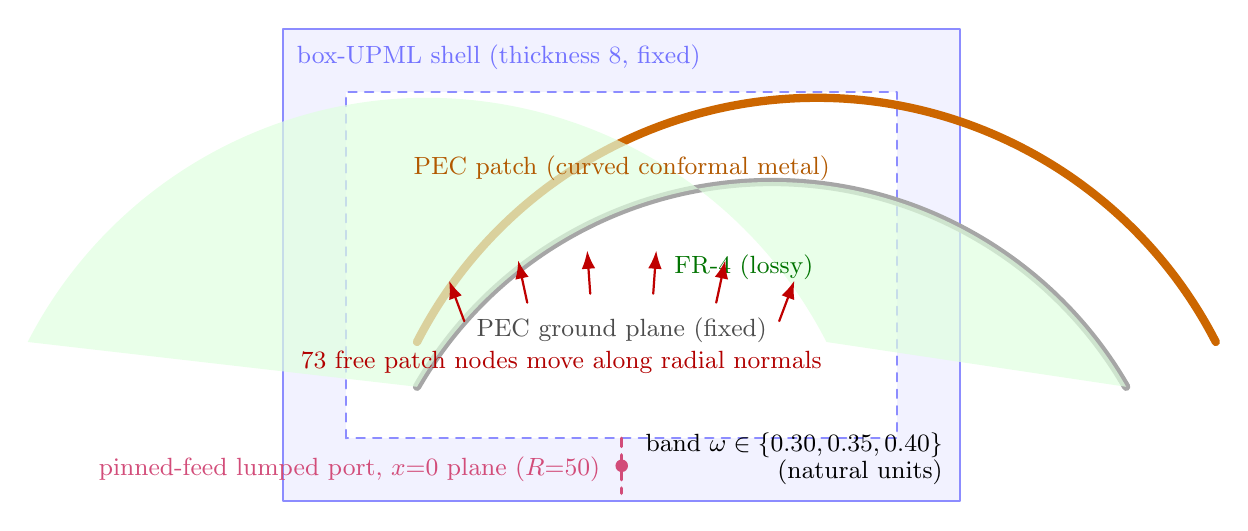
\begin{tikzpicture}[>=Latex,line join=round,line cap=round]

  % ---- matched box-UPML absorber shell (outer, held fixed) --------------
  \draw[fill=blue!5,draw=blue!45,thick]
        (-4.3,-3.0) rectangle (4.3,3.0);
  \draw[fill=white,draw=blue!45,thick,dashed]
        (-3.5,-2.2) rectangle (3.5,2.2);
  \node[blue!55,anchor=north west,font=\small]
        at (-4.25,2.92) {box-UPML shell (thickness $8$, fixed)};

  % ---- curved conformal FR-4 + PEC slab (wrapped about the y-axis) ------
  % A circular arc of illustrative bend radius stands in for the cylinder of
  % bend_radius = 40 (natural units). PEC patch = outer arc, ground = inner arc.
  \def\Rc{5.2}          % illustrative draw radius (NOT the 40 natural-unit value)
  \def\cx{0}
  \def\cy{-6.05}        % arc center below the frame, so the visible arc is gentle
  % ground plane (inner arc, PEC, held fixed)
  \draw[draw=gray!70,line width=3pt]
        (\cx-2.6,{\cy+sqrt(\Rc*\Rc-2.6*2.6)})
        arc[start angle={180-asin(2.6/\Rc)}, end angle={asin(2.6/\Rc)}, radius=\Rc];
  % patch conductor (outer arc, PEC) -- the movable boundary
  \def\Ro{5.7}
  \draw[draw=orange!80!black,line width=3pt]
        (\cx-2.6,{\cy+sqrt(\Ro*\Ro-2.6*2.6)})
        arc[start angle={180-asin(2.6/\Ro)}, end angle={asin(2.6/\Ro)}, radius=\Ro];
  % FR-4 dielectric fill between the two arcs (schematic band)
  \fill[green!12,opacity=0.7]
        (\cx-2.6,{\cy+sqrt(\Rc*\Rc-2.6*2.6)})
        arc[start angle={180-asin(2.6/\Rc)}, end angle={asin(2.6/\Rc)}, radius=\Rc]
        -- (\cx+2.6,{\cy+sqrt(\Ro*\Ro-2.6*2.6)})
        arc[start angle={asin(2.6/\Ro)}, end angle={180-asin(2.6/\Ro)}, radius=\Ro]
        -- cycle;

  \node[orange!70!black,anchor=south,font=\small] at (0,0.95)
        {PEC patch (curved conformal metal)};
  \node[green!45!black,anchor=north,font=\small] at (1.55,0.25)
        {FR-4 (lossy)};
  \node[gray!60!black,anchor=north,font=\small] at (0,-0.55)
        {PEC ground plane (fixed)};

  % ---- radial-normal design DOFs: arrows off the patch arc --------------
  \foreach \a in {-2.0,-1.2,-0.4,0.4,1.2,2.0}{
     \pgfmathsetmacro\yy{\cy+sqrt(\Ro*\Ro-\a*\a)}
     \pgfmathsetmacro\ang{atan2(\yy-\cy,\a)}
     \draw[->,red!75!black,thick]
        (\a,\yy) -- ++({0.55*cos(\ang)},{0.55*sin(\ang)});
  }
  \node[red!70!black,anchor=south west,font=\small] at (-4.2,-1.5)
        {$73$ free patch nodes move along radial normals};

  % ---- pinned-feed lumped port on the x=0 plane -------------------------
  \draw[purple!70,line width=1.2pt,dashed] (0,-2.2) -- (0,-2.9);
  \node[purple!70,circle,fill=purple!70,inner sep=1.6pt] at (0,-2.55) {};
  \node[purple!70,anchor=east,font=\small] at (-0.15,-2.6)
        {pinned-feed lumped port, $x{=}0$ plane ($R{=}50$)};

  % ---- band + objective annotation (all from the TOML) ------------------
  \node[anchor=south east,font=\small,align=right] at (4.2,-2.92)
        {band $\omega\in\{0.30,0.35,0.40\}$\\[-1pt]
         (natural units)};

\end{tikzpicture}
\end{document}
